\section{L11-Convezione}
\subsection{Introduzione}
La \textbf{convezione} identifica il trasporto di energia associato al
moto macroscopico del sistema: è quindi un processo che si
verifica tra la superficie di un corpo ed un fluido in moto
relativo.\newline
Si può classificare in due tipologie:
\begin{itemize}
    \item \textbf{Convezione forzata}: il moto del fluido è imposto da un agente esterno (per es. un ventilatore);
    \item \textbf{Convezione naturale} (solo all'interno di un campo gravitazionale): il moto del fluido è causato dal processo di trasmissione del calore che causa spinte di galleggiamento (per via delle differenze di densità).
\end{itemize}
\subsubsection{Fluidodinamica}
Per poter determinare il valore di scambio termico $h$, dobbiamo capire come si muove un fluido attorno all'oggetto studiato (cioè attorno a una parete).\newline
\newline
La trasmissione del calore per convezione è \textbf{fortemente legata} alla dinamica del
fluido che lambisce la parete solida.
\begin{itemize}
    \item In molte situazioni il moto del fluido \textbf{non assume una soluzione analitica}
    (natura tridimensionale e non lineare);
    \item Per questa ragione l’approccio utilizzato è di tipo \textbf{sperimentale} con
    l’introduzione di una \textbf{legge fenomenologica}
    \[
        \frac{\delta \rho}{\delta t} + \nabla \cdot (\rho \vec{u}) = 0
    \]
    \[
        \frac{\delta \rho \vec{u}}{\delta t} + \nabla \cdot  (\rho \vec{u} \vec{u}) = - \nabla P + \nabla \cdot \left[\mu \left(\nabla \vec{u} + \nabla \vec{u}^T\right)\right]
    \]
    per via di $ \nabla \cdot \rho \vec{u} \vec{u}$ si ha una non linearità. Queste espressioni sono molto difficili da anlizzare, e perciò, a parte per pochissimi casi particolari, non si riesce ad avere una soluzione analitica, cioè queste equazioni spesso non si riescono a risolvere.
\end{itemize}
\subsubsection{Legge di Newton}
\[
    J = h (T_p - T_f)
\]
dove \newline
$h =$ coefficiente di scambio termico convettivo $[W/m^2 K]$\newline
$T_p =$ temperatura della parete solida $[K]$\newline
$T_f =$ temperatura del fluido $[K]$
\subsubsection{coefficiente di scambio termico convettivo}
Tutta la complessità delle equazioni del paragrafo precedente è concentrata all'interno del parametro $h$ (coefficiente di scambio termico convettivo).\newline
Il coefficiente di scambio convettivo (o conduttanza convettiva) dipende da:
\begin{itemize}
    \item proprietà fisiche del fluido;
    \item dinamica del flusso;
    \item geometria della superficie della parete.
\end{itemize}
\ \newline
\textbf{Valori generici del coefficiente convettivo}:\newline
\[
    \begin{matrix}
        \text{gas stagnante}\; & 5-50 \; [W/m^2K]\\
        \text{acqua stagnante}\;& 100 \; [W/m^2K]\\
        \\
        \text{gas in moto}\; & 15-1000 \; [W/m^2K]\\
        \text{olio minerale}\; & 50-3000\; [W/m^2K]\\
        \text{acqua in moto}\; &200-10000\; [W/m^2K]\\
        \\
        \text{acqua in ebollizione o condensazione}\; &1000-100000\; [W/m^2K]\\
        \text{metalli liquidi}\; &10000-100000\; [W/m^2K]\\
    \end{matrix}
\]
\subsubsection{Temperatura del fluido}
Non è facile attribuire un ben preciso valore per $T_f$ nella legge di Newton, in
quanto il fluido è generalmente sede di un gradiente termico e la sua temperatura
varia da punto a punto.
\begin{itemize}
    \item L’esperienza mostra che il gradiente termico è particolarmente accentuato
    nello strato di fluido direttamente a contatto con la parete (detto \textbf{strato limite
    termico})
    \item I criteri di scelta o definizione di $T_f$ risulteranno in generale quelli della
    \textbf{semplicità} di determinazione e di \textbf{significatività}
    \item Le definizioni di $T_f$ saranno diverse per ogni configurazione geometrica
    \item Nel caso di un fluido che lambisce esternamente un corpo solido (\textbf{convezione
    esterna}), si utilizza come temperatura $T_f$ la cosiddetta \textbf{temperatura
    asintotica} $T_\infty$ (lontano dalla parete, dove la temperatura è praticamente costante), ovvero la temperatura del fluido misurata in un punto in cui è
    praticamente nulla l’influenza della parete del solido
    \item Nel caso invece di un fluido che scorre all’interno di un condotto (\textbf{convezione
    interna}) si possono adottare diverse soluzioni anche se è maggiormente
    diffuso l’utilizzo della \textbf{temperatura di miscelamento adiabatico}, definita
    come:
    \[
        T_m = \frac{\int_{S}\rho c_P T w dS}{\int_{S}\rho c_P w dS}
    \]
    con $\rho$ massa volumica del fluido $[kg/m^3]$, $c_P$ calore specifico del fluido $[j/kgK]$, $w$ velocità del fluido $[m/s]$, $S$ sezione del condotto $[m^2]$.
\end{itemize}
\subsubsection{Il moto dei fluidi: esempio della lastra piana}
Poichè la convezione del calore è strettamente legata allaa fluidodinamica, è essenziale chiarire alcuni aspetti fenomenologici, in particolare il regime di flusso. Quando si ha un fluido che fluisce attorno a un oggetto all'interno di un condotto, quello che succede è che in funzione della velocità della corrente del fluido, possiamo trovare due situazioni:
\begin{itemize}
    \item il flusso è laminare: i vari strati del fluido scorrono nello spazio in maniera "ordinata", senza oscillazioni, e senza miscugli fra i vari strati.
    \item Se si alza la velocità del fluido, si trova un altroregime di flusso, cioè il flusso turbolento, in cui i vari strati oscillano e si creano una serie di vortici e moti disordinati.
\end{itemize}
per quanto riguarda la trasmissione del calore, che si occupa dell ostudio degli scambi di calore fra un fluido in movimento e una parete solida, possiamo studiare il problema della latra piana non in movimento:
\begin{center}
    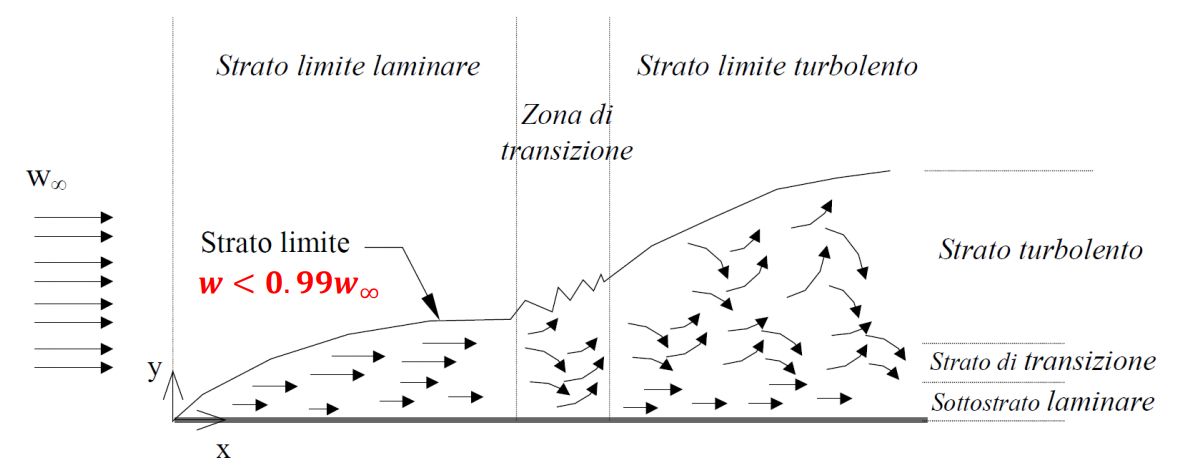
\includegraphics[height=5cm]{../L11/img1.PNG}
\end{center}
La velocità $w_{\infty}$ rappresenta la velocità del flusso lontano dalla parete (linea nera spessa inferiore). Lontano dalla parete il flusso può essere turbolento o meno, la cosa non è di nostro interesse, ciò che importa è il comprotamento del fluido a contatto con la lastra.\newline
I filetti di fluido che scorrono in prossimità della parete devono adattarsi alle condizioni di aderenza con la parete: siccome la parete non si muove, anche il fluido adiacenti al fluido non si devono muovere. Dunque la velocità del flusso passa da $w_{\infty}$ e $0$. Appena ci spostiamo leggermente dalla parete notiamo che anche qui i filetti di fluido vengono rallentati a causa della presenza del fluido a velocità $0$ (c'è una sorta di attrito causato dalla viscosità del fluido). Quindi la velocità $w_{\infty}$ del flusso, più ci si avvicina alla parete più è lenta fino a raggiungere la velocità $0$ quando è a contatto diretto con la parete. Si chiama zona di \textbf{strato limite} la zona in cui la velocità del fluido $w < 0.99 w_{\infty}$.\newline
\newline
All'inizio l'interazione fra i vari strati fluidi è stabile, quindi all'inizio il movimento del fluido nello strato limite è laminare. Più si continua a percorrere la parete il movimento del fluido nello strato limite inizia a essere instabile, e, superata una certa soglia, si raggiunge una zona di strato limite turbolento in cui il fluido è completamente instabile. All'interno dello strato limite turbolento ci sono tre aree: in prossimità della parete si ha un sottostrato laminare (la parete ha un effetto stabilizzante), in seguito si trova uno strato di transizione e uno strato turbolento.\newline
\newline
Questa fenomenologia del moto dei fluidi implica che, all'inizio, nello strato limite laminare, ci sarà uno scambio termico "facile", i filetti fluidi sono ordinati e non c'è uno spostamento verticale dei filetti del fluido. Nel caso turbolento invece i filetti che sono inizialmente a contatto con la parete dopo aver scambiato calore, possono spostarsi "verticlamente" (nell immagine) e allontanarsi dalla parete, c'è quindi una sorta di trasporto di massa verticale.\newline
\newline
Per quanto riguarda il coefficiente convettivo: nella zona laminare $h$ ha un determinato valore e nella zona turbolenta questo coefficiente $h$ subirà un notevole incremento (dovuto allo scambio di massa verticale fra i vari filetti di fluido).\newline
\newline
Video dimostrativo: \url{https://www.youtube.com/watch?v=wXsl4eyupUY}
\newline
\begin{itemize}
    \item Negli strati adiacenti allo strato aderente alla lastra le particelle del fluido per
    effetto della viscosità tenderanno progressivamente a raggiungere la velocità
    indisturbata $w_{\infty}$. In questi strati sono influenti le sollecitazioni di taglio viscose
    (attrito) e la regione in cui la velocità è inferiore alla velocità indisturbata è
    detta zona di \textbf{strato limite} ($w < 0,99 w_{\infty}$).
    \item Un moto è denominato \textbf{laminare} se ordinato (o stabile) ovvero se i singoli filetti fluidi si muovono tutti parallelamente tra loro.
    \item Un moto è denominato \textbf{turbolento} se caratterizzato da variazioni di velocità e moto disordinato (o instabile) con componenti di velocità trasversali (vortici).
    \item In generale la \textbf{transizione} tra moto laminare e turbolento non avviene bruscamente ma esiste una regione nella quale il moto fluttua tra laminare e turbolento prima di diventare completamente instabile e perciò turbolento.
    \item La dimostrazione sperimentale dell'esistenza di diversi \textbf{regimi di moto} è dovuta a \textbf{Osborne Reynolds} che nel 1880 eseguì una serie di esperienze al fine di comprendere come si potesse descrivere il movimento di un fluido.
\end{itemize}
\subsection{Convezione forzata}
\subsubsection{L'analisi dimensionale}
Il coefficiente convettivo nel caso di \textbf{convezione forzata} dipende da:
\begin{itemize}
    \item le caratteristiche del fluido: densità ($\rho$), viscosità ($\mu$), calore specifico a pressione costante ($c_P$), conduttività termica ($k$);
    \item dalle condizioni di moto del fluido: velcoità caratteristica ($w$);
    \item dalla geometria della parete: lunghezza caratteristica ($\lambda$).
\end{itemize}
\[
    h = h(\rho, \mu, c_P, k , w , \lambda)
\]
(nota: $h$ \textbf{non è una proprietà della materia}).\newline
\newline
Si hanno $r= 7$ grandezze fisiche ($h, \rho, \mu, c_P, k , w , \lambda$) e $n = 4$ grandezze fondamentali ($L,M,t,T$). \newline
\newline
Dal \textbf{teorema di buckingham} (dispensa sezione $6.4$), si dovrà avere un legame tra $\Pi = r - n = 3$ \textbf{gruppi adimensionali}.\newline
\newline
Esiste una relazione funzionale (da determinare sperimentalmente) tra questi $3$ gruppi adimensionali
\[
    g'(\pi_1, \pi_2, \pi_3) = 0
\]
\textbf{Gruppi adimensionali per convezione forzata}:
\[
    Nu = \frac{h\lambda}{k} \;\;\;\;\; \text{numero di Nusselt}
\]
\[
    Re = \frac{\rho w \lambda}{\mu} \;\;\;\;\;\text{numero di Reynolds}
\]
\[
    Pr = \frac{c_P \mu}{k} \;\;\;\;\;\text{numero di Prandtl}
\]
\subsubsection{Numero di Nusselt}
\[
    Nu = \frac{h\lambda}{k}
\]
Può essere interpretato come \textbf{rapporto} tra la potenza termica
scambiata con moti macroscopici (\textbf{convezione}) e la potenza
termica scambiata per \textbf{conduzione} nello strato limite. \newline
\newline
In effetti, dividendo il flusso di calore per convezione ($h \Delta T$)
per il flusso di calore per conduzione ($k / \lambda \cdot \Delta T$) si ottiene
il numero di Nusselt
\[
    Nu = \frac{h\Delta T}{\frac{k}{\lambda}\Delta T}
\]
Indica di quanto è stato incrementato lo scambio termico
per via del moto del fluido.\newline
\newline
Non è mai minore di $1$.
\subsubsection{Numero di Reynolds}
\[
    Re = \frac{\rho w \lambda}{\mu}
\]
Può essere interpretato come rapporto tra la risultante
delle forze di inerzia e la risultante delle forze viscose
\[
    Re = \frac{\text{Forze d'inerzia}}{\text{Forze viscose}} = \frac{\rho w \frac{\delta w}{\delta x}}{\mu \frac{\delta ^2 w}{\delta y^2}} \propto \frac{\rho w \frac{w}{\lambda}}{\mu \frac{w}{\lambda^2}}
\]
Indica se il moto è in regime laminare o turbolento (Reynolds critico).
\begin{itemize}
    \item Flussso interno a un condotto ($\lambda = D_i, w = w_m$):\newline
    $Re_D < 2000$, moto laminare;\newline
    $Re_D > 4000$, moto turbolento;
    \item Moto lungo una lastra piana ($\lambda = x, w = w_\infty$):\newline
    $Re_x < 3,5 \cdot  10^5$, moto laminare; \newline
    $Re_x > 3,5 \cdot  10^5$, moto turbolento;
    \item Moto attorno ad un cilindro ($\lambda = D_e, w = w_\infty$):\newline
    $Re_D < 2,8 \cdot  10^5$, moto laminare;\newline
    $Re_D > 2,8 \cdot  10^5$, moto tubrolendo;
\end{itemize}
Attenzione: valori limiti variabili in funzione di molti altri parametri secondari.
\subsubsection{Numero di Prandtl}
\[
    Pr = \frac{c_P \mu}{k}
\]
Può essere interpretato come rapporto tra la viscosità cinematica, $v = \mu/\rho$, (da cui dipende la diffusione della quantità di moto) e la diffusività termica del fluido, $a = k / \rho c_P$ (da cui dipende la diffuzione molecolare della potenza termica).
\[
    Pr = \frac{\rho c_P}{k} \frac{\mu}{\rho}
\]
gas: fra $0,7$ e $1$\newline
acqua: fra $2$ e $10$ \newline
metalli liquidi: fra $0,005$ e $0,03$\newline
oli pesanti: fra $100$ e $100000$\newline
\newline
\textbf{Indica lo spessore relativo dello strato limite termico rispetto a quello fluidodinamico}.
\subsubsection{Forma monomia}
La relazione tra i gruppi adimensionali è espressa tramite una forma monomia 
\[
    Nu = A R e^\alpha Pr^\beta
\]
I coefficienti $A, \alpha, \beta$ devono essere determinati attraverso l'interpolazione di risultati di prove sperimentali.\newline
\newline
I numeri adimensionali dipendono da parametri termofisici che normalmente a
loro volta dipendono dalla temperatura (e talvolta anche dalla pressione) alla
quale avviene il fenomeno di convezione. Diventa quindi importante stabilire a
\textbf{quale temperatura} devono essere valutati i suddetti parametri.
\subsubsection{Temperature}
Le proprietà termofisiche si possono valutare in condizioni differenti:
\begin{itemize}
    \item Alla temperatura di parete $T_P$,
    \item Alla temperatura asintotica $T_\infty$,
    \item Alla temperatura di film $T_{film} = \frac{T_P + T_\infty}{2}$,
    \item Alla temperatura di miscelamento adiabatico (temperatura media dal punto di vista energetico) $T_m = \frac{\int_S \rho w c_P T dS}{\int_S \rho w c_P dS}$
\end{itemize}
\subsubsection{Alcune correlazioni}
Convenzione \textbf{forzata}: flusso su lastra piana a $T_P$  costante:
\begin{itemize}
    \item Se strato limite laminare sull'intera lastra $(L<x_c)$ e se $P_r \geq 0,6$:\newline
    $h = h(x)$ locale: $Nu_x = 0,332 Re_x^{0,5}Pr^{1/3}$\newline
    $h$ medio: $\bar{Nu} = 0,664Re_L^{0,5}Pr^{1/3}$
    \item Se strato limite turbolento sull'intera lastra ($x_c << L$) e se $0,6 \leq Pr \leq 60$:\newline
    $h = h(x)$ locale: $Nu_x = 0,0296Re_x^{0,8} Pr^{1/3}$\newline
    $h$ medio: $\bar{Nu} = 0,037 Re_L^{0,8} Pr^{1/3}$
\end{itemize}
\ \newline
\rule{\textwidth}{0,4pt}
Convenzione \textbf{forzata}: flusso esterno su cilindri a $T_P$ costante:\newline
Relazione di Churchill e Bernstein (cilindro singolo liscio)
\[
    Nu_D = 0,3 + \frac{0,62Re^{0,5Pr^{1/3}}}{\left[1 + \left(\frac{0,4}{Pr}\right)^{\frac{2}{3}}\right]^{\frac{1}{4}}}\cdot \left[1 + \left(\frac{Re}{28200}\right)^{\frac{5}{8}}\right]^{\frac{4}{5}}\;\;\;\;\;\;\;\;\;\;\;\;\;\;\;Re \cdot Pr > 0,2
\]
Le proprietà termofisiche sono valutate alla temperatura di film.\newline
\newline
\rule{\textwidth}{0,4pt}
Convezione \textbf{forzata}: flusso esterno su cilindri a $T_P$ costante:\newline
relazione di Hilpert (cilindro singolo liscio)
\[
    Nu_D = C Re^m Pr^{1/3}
\]
\begin{center}
    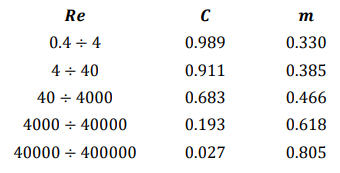
\includegraphics[height=3cm]{../L11/img2.PNG}
\end{center}
\ \newline
\rule{\textwidth}{0,4pt}
Convezione \textbf{forzata}: moto sviluppato all'interno di un condotto circolare:\newline
\[
    Nu_D = 3,66 \;\;\;\;\; \text{moto laminare con $T_P$ costante}\;
\]
\[
    Nu_D = 4,36 \;\;\;\;\; \text{moto laminare con $J$ costante}\;
\]
\[
    Nu_D = 0,23 Re^{0,8}Pr^n \;\;\;\;\; \text{moto turbolento (relazione di Dittus-Boelter)}\;\begin{cases}
        Re > 10000 \;\; 0,7< Pr, 160\\
        n = 0,3 \; \text{fluido in raffreddamento}\\
        n = 0,4 \; \text{fluido in riscaldamento}
    \end{cases}
\]
\[
    Nu_D = 0,027 Re^{0,8} Pr^{1/3}\left(\frac{\mu}{\mu_P}\right)^{0,14}\;\;\;\;\; \text{moto turbolento (relazione di Sieder-Tate)} \;\begin{cases}
        re > 10000\\
        0,7 < Pr< 16700\\
        \mu_P = \mu(T_P)
    \end{cases}
\]
Le proprietà termofisiche sono valutate alla temperatura di miscelamento adiabatico.
\subsubsection{Flusso all'interno di tubi}
In ogni sezione: $w$ varia da un valore pari a zero sulla parete a un valore
massimo sull’asse del tubo. \newline
\newline
In ogni sezione: $T$ varia da un valore pari a quello che si rileva sulla parete a
un valore maggiore o inferiore (a seconda che il processo sia di
raffreddamento o di riscaldamento) sull’asse del tubo.\newline
\newline
$T$ e $w$ si assumono comunque costante per ogni sezione e pari al loro valore
medio. Ovviamente questi valori medi possono variare lungo l’asse del tubo.
\newline
\begin{itemize}
    \item La velocità media si determina col principio di conservazione della massa $\dot{m} = \rho w_m S$.
    \item La temperatura media si determina col principio di conservazione dell'energia (temperatura adiabatica di miscelamento).
\end{itemize}
\ \newline
Esistono due principali tipologie di problemi (semplificati):
\begin{itemize}
    \item Il flusso termico superficiale è costante $J =$ costante;
    \item La temperatura della parete è costante $T_P =$ costante.
\end{itemize}
Non possono essere contemporaneamente presenti ambedue le condizioni.\newline
\newline
Il flusso termico è dato da $J = h (T_P - T_m)$.\newline
\newline
\textbf{Caso flusso termico superficiale costante} ($J =$ costante):
\begin{center}
    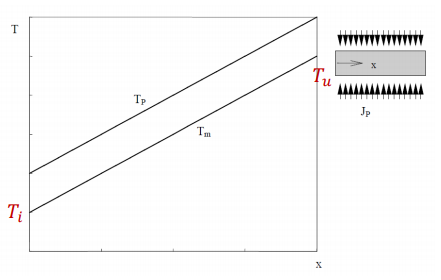
\includegraphics[height=3cm]{../L11/img3.PNG}
\end{center}
\[
    \dot{Q} = JS = \dot{m} c_P (T_u- T_i)
\]
\[
    T_u = T_i + \frac{JS}{\dot{m} c_P}
\]
\[
    J = h (T_P - T_m)
\]
\ \newline
\textbf{Caso temperatura della parete costante} ($T_P =$ costante):
\begin{center}
    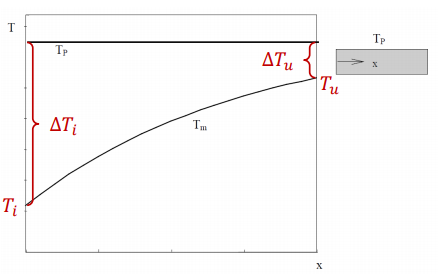
\includegraphics[height=3cm]{../L11/img4.PNG}
\end{center}
\[
    \dot{Q} = JS = \dot{m} c_P (T_u - T_i)
\]
\[
    T_u = T_i + \frac{JS}{\dot{m}c_P}
\]
\[
    J = h \Delta T_{ml} = h \frac{\Delta T_u - \Delta T_i}{ln \left(\frac{\Delta T_u}{\Delta T_i}\right)}
\]
\subsection{Convezione naturale}
\subsubsection{L'analisi dimensionale}
Invece di avere la velocità del fluido abbiamo $g \beta \Delta T$, che sono le spinte di galleggiamento:
\[
    h = h(\rho, \mu, c_P, k, g \beta \Delta T, \lambda)
\]
Si hanno $r = 7$ grandezze fisiche ($h, \rho, \mu, c_P, k, g \beta \Delta T, \lambda$) e $n = 4$ grandezze fondamentali ($L, M, t, T$).\newline
\newline
Dal \textbf{teorema di Buckingham} (dispensa sezione $6.4$), si dovrà avere un legame tra $\Pi = r-n = 3$ \textbf{gruppi fondamentali}.\newline
\newline
Esiste una relazione funzionale (da determinare sperimentalmente) tra questi $3$ gruppi adimensionali:
\[
    g'(\pi_1, \pi_2, \pi_3) = 0
\]
\textbf{Gruppi adimensionali per convezione naturale}
\[
    Nu = \frac{h \lambda}{k} \;\;\;\;\;\text{Numero di Nusselt}
\]
\[
    Gr = \frac{\rho^2 g \beta \Delta T \lambda^3}{\mu^2} \;\;\;\;\;\text{Numero di Grashoff}
\]
\[
    Pr = \frac{C_P \mu}{k} \;\;\;\;\; \text{Numero di Prandtl}
\]
\subsubsection{Numero di Grashoff}
\[
    Gr = \frac{\rho^2 g \beta \Delta T \lambda^3}{\mu^2}
\]
Può essere interpretato come \textbf{rapporto} tra il prodotto delle forze di \textbf{galleggiamento} e di inerzia ed il quadrato della risultante delle forze \textbf{viscose}.
\[
    Gr = \frac{F_{galleggiamento}F_{inerzia}}{F_{viscose}^2} = \frac{\rho g \beta \Delta T \left(\rho w \frac{\delta w}{\delta x}\right)}{\left(\mu \frac{\delta^2 w}{\delta y^2}\right)^2} \propto \frac{\rho g \beta \Delta T \rho w \frac{w}{\lambda}}{\mu^2 \frac{w^2}{\lambda^4}}
\]
\textbf{Indica se il moto è in regime laminare o turbolento (Grashoff critico)}.
\subsubsection{Peclet e Rayleigh}
\textbf{Convezione forzata}:
\[
    Pe = Re \cdot Pr = \frac{w \lambda}{a} \;\;\;\;\;\text{Numero di Peclet (poco usato)}
\]
\textbf{Convezione naturale}:
\[
    Ra = Gr \cdot Pr = \frac{g \beta \Delta T \lambda^3}{a v} \;\;\;\;\; \text{Numero di Rayleigh (spesso usato)}
\]
Spesso viene usato il numero di Rayleight al posto del numero di Grashoff e di Prandtl.\newline
\newline
Il numero di Rayleigh ha la stessa funzione del numero di raynolds per la convezione forzata, cioè \textbf{determinare il regime di moto}.
\subsubsection{Considerazioni}
Il coefficiente $h$ dipende:
\begin{itemize}
    \item dalle caratteristiche del fluido: come nel caso della convezione forzata, ma in
    più abbiamo il coefficiente di dilatazione termica a pressione costante $\beta$ da cui
    dipende il cambiamento di densità;
    \item dalle condizioni di moto del fluido: la velocità del fluido varia localmente e
    dipende dalle spinte di galleggiamento $f_g \sim \rho g \beta (T_P- T_{\infty})$;
    \item dalla geometria della parete: come nel caso precedente ma con la necessità di
    conoscere la posizione della parete rispetto al campo gravitazionale.    
\end{itemize}
Le proprietà termofisiche sono valutate alla temperatura di film
\subsubsection{Alcune correlazioni}
\begin{center}
    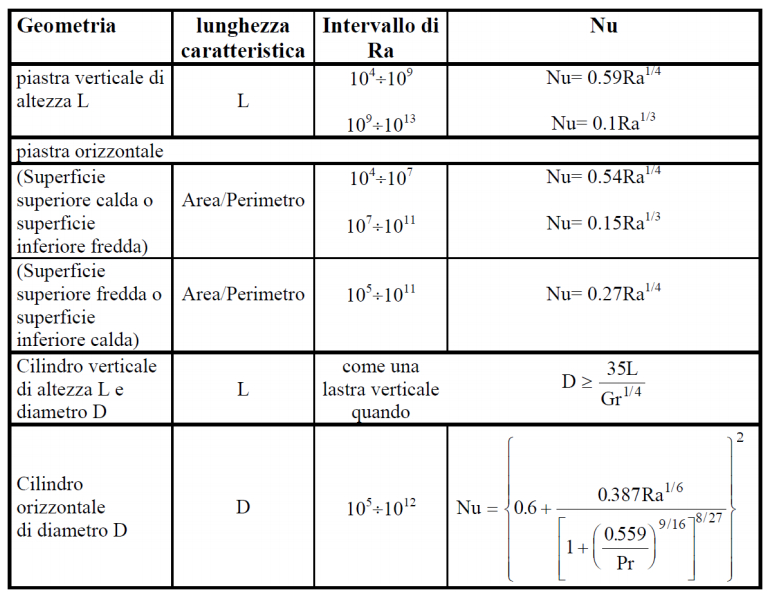
\includegraphics[height=6cm]{../L11/img5.PNG}
\end{center}
Le proprietà termofisiche sono valutate alal temperatura di film